\section{Arquitetura}

Nessa seção do capítulo, apresenta-se a arquitetura da aplicação, que define como os componentes do sistema interagem entre si e com o usuário.

\subsection{Definições da arquitetura}

O sistema foi estruturado com base no modelo cliente-servidor, no qual o front-end e o back-end operam como aplicações independentes que se comunicam por meio de requisições HTTP, seguindo a arquitetura RESTful.

O back-end é responsável pelo processamento da lógica de negócios e pela persistência dos dados, enquanto o front-end realiza a apresentação e interação com o usuário. Essa separação garante maior modularidade e facilita a manutenção da aplicação, cujo domínio é um ambiente de \textit{coworking} para salões de beleza.

A arquitetura do sistema adota um padrão baseado no Model-View-Controller (MVC) de forma adaptada, aproximando-se de uma arquitetura em camadas. Cada camada possui uma responsabilidade bem definida, conforme descrito a seguir:

\begin{itemize}
  \item \textbf{Controller:} Responsável por receber e tratar as requisições provenientes do cliente (front-end), encaminhando-as para a camada de serviço correspondente. Esta camada lida diretamente com aspectos de infraestrutura externa, como servidores de borda e APIs públicas.
  \item \textbf{Service:} Centraliza a lógica de negócio da aplicação. É responsável por processar as regras do domínio e pode tanto consumir outras funções de serviço quanto interagir com a camada de persistência.
  \item \textbf{Repository:} Trata das operações relacionadas à persistência de dados. Atua como uma interface entre os serviços e os mecanismos de armazenamento, como bancos de dados relacionais ou caches, promovendo o desacoplamento da lógica de negócio em relação à camada de dados.
\end{itemize}

\subsection{Diagrama da arquitetura}

Esta subseção apresenta dois diagramas que representam a arquitetura do sistema desenvolvido: o diagrama de componentes e o diagrama de implantação. Esses diagramas auxiliam na visualização do relacionamento entre as partes da aplicação, bem como a sua distribuição nos ambientes computacionais.

\subsubsection{Diagrama de componentes}


O diagrama de componentes representa a organização lógica dos principais módulos da aplicação, evidenciando as dependências e as formas de comunicação entre eles. Ele demonstra como os componentes interagem por meio de interfaces — que definem contratos de uso — e implementações — que oferecem as funcionalidades esperadas.

Esse tipo de diagrama é útil para visualizar a estrutura modular da aplicação, facilitando o entendimento da separação de responsabilidades e da reutilização de código, além de apoiar decisões relacionadas à manutenção e evolução do sistema.

\begin{figure}[htb]
  \centering
  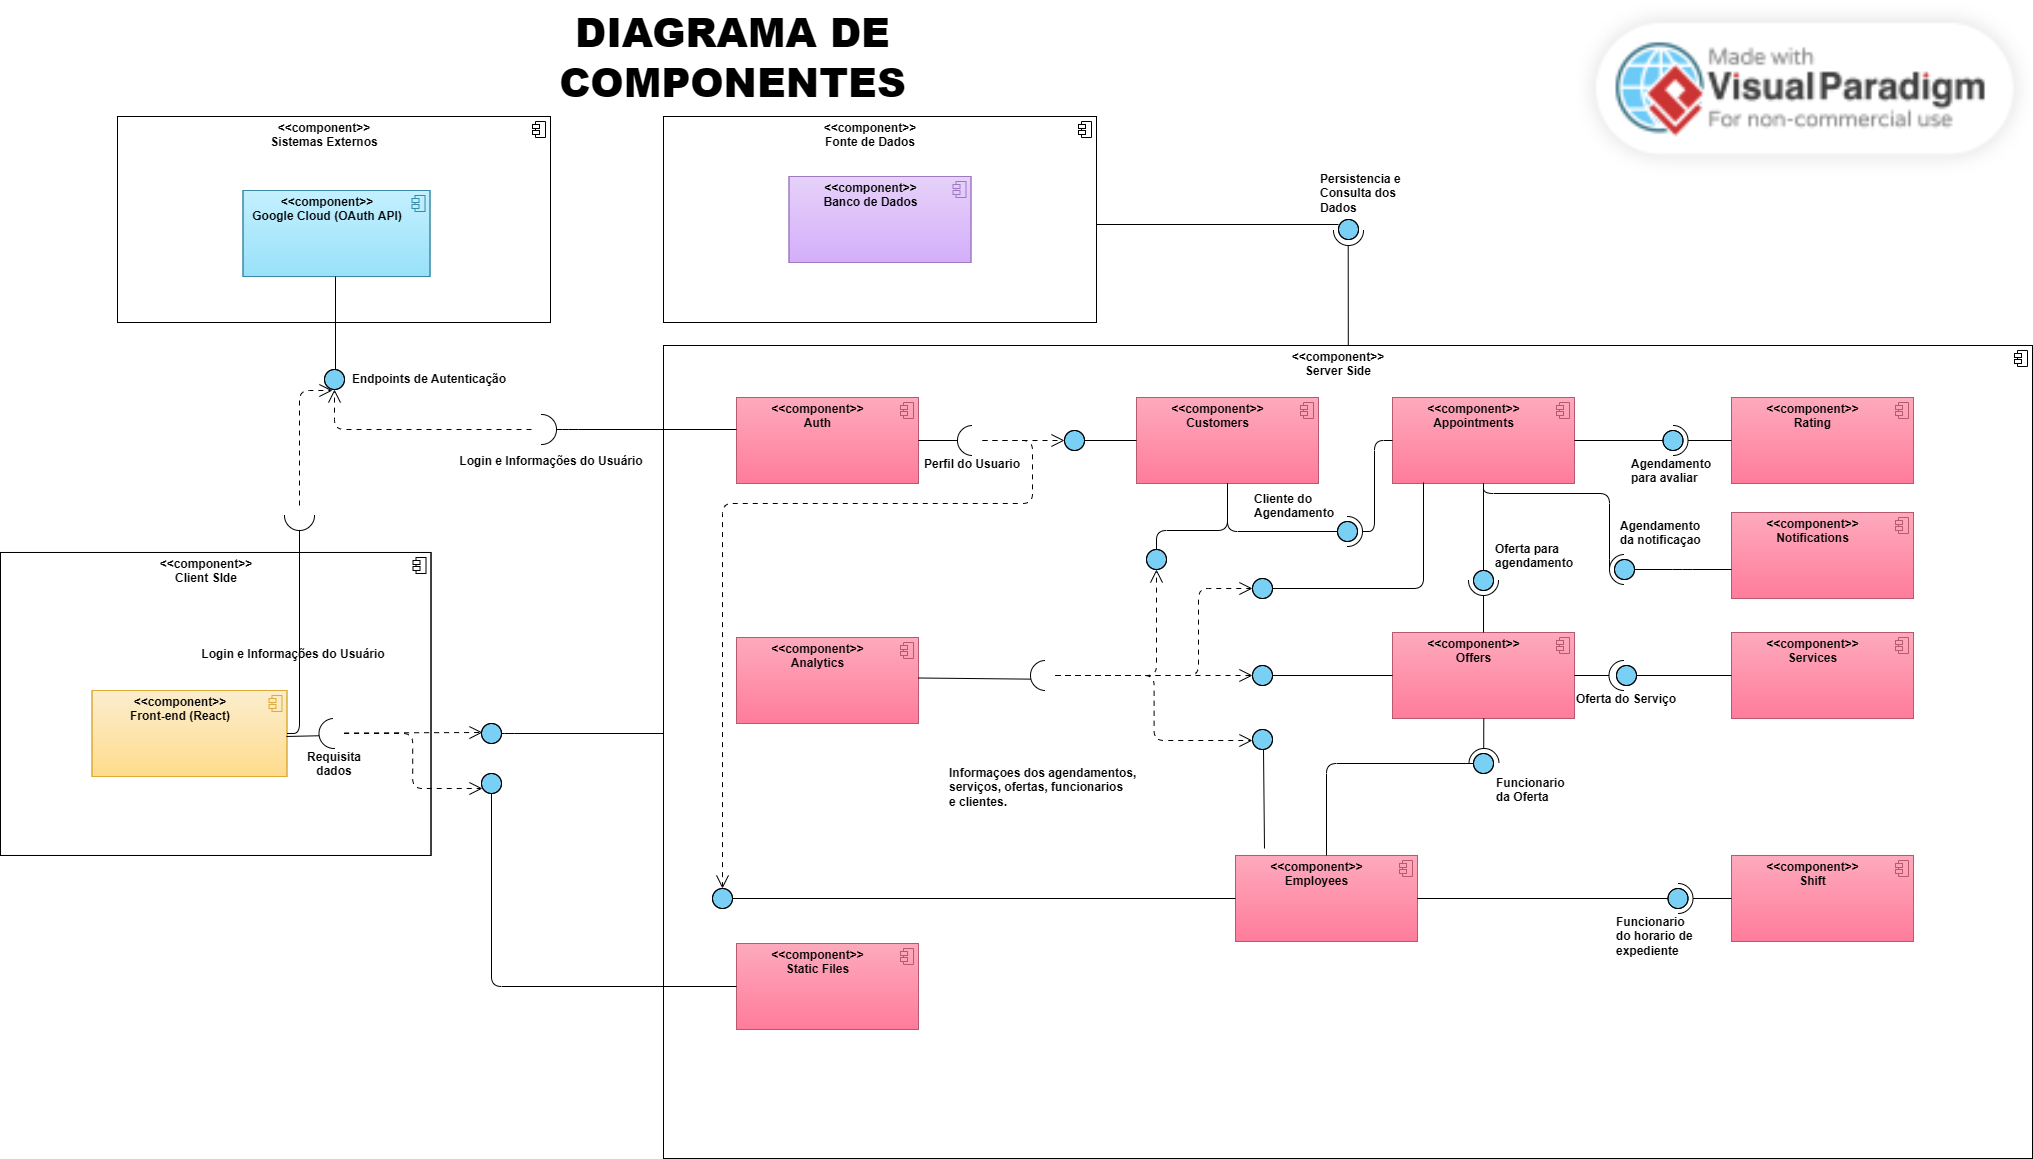
\includegraphics[width=\textwidth]{cap04-desenvolvimento/images/4-3-2-1-diagrama-componentes}
  \caption{Diagrama de componente da aplicação}
  \label{fig:diagrama-componente}
\end{figure}

\subsubsection{Diagrama de Implantação}

O diagrama de implantação mostra como os componentes do sistema estão distribuídos em termos de infraestrutura, seja em servidores físicos ou ambientes virtuais. Ele ajuda a entender onde cada parte da aplicação está rodando, como os serviços se conectam entre si e quais recursos são necessários para que tudo funcione bem em produção.

Esse tipo de representação é especialmente útil para quem for implantar ou manter o sistema, pois facilita a visualização de elementos como servidores, banco de dados, gateways de rede, e outras dependências da aplicação. Além disso, o diagrama contribui para o planejamento de permissões, acessos e políticas de segurança que precisam ser configuradas na infraestrutura.

\begin{figure}[htb]
  \centering
  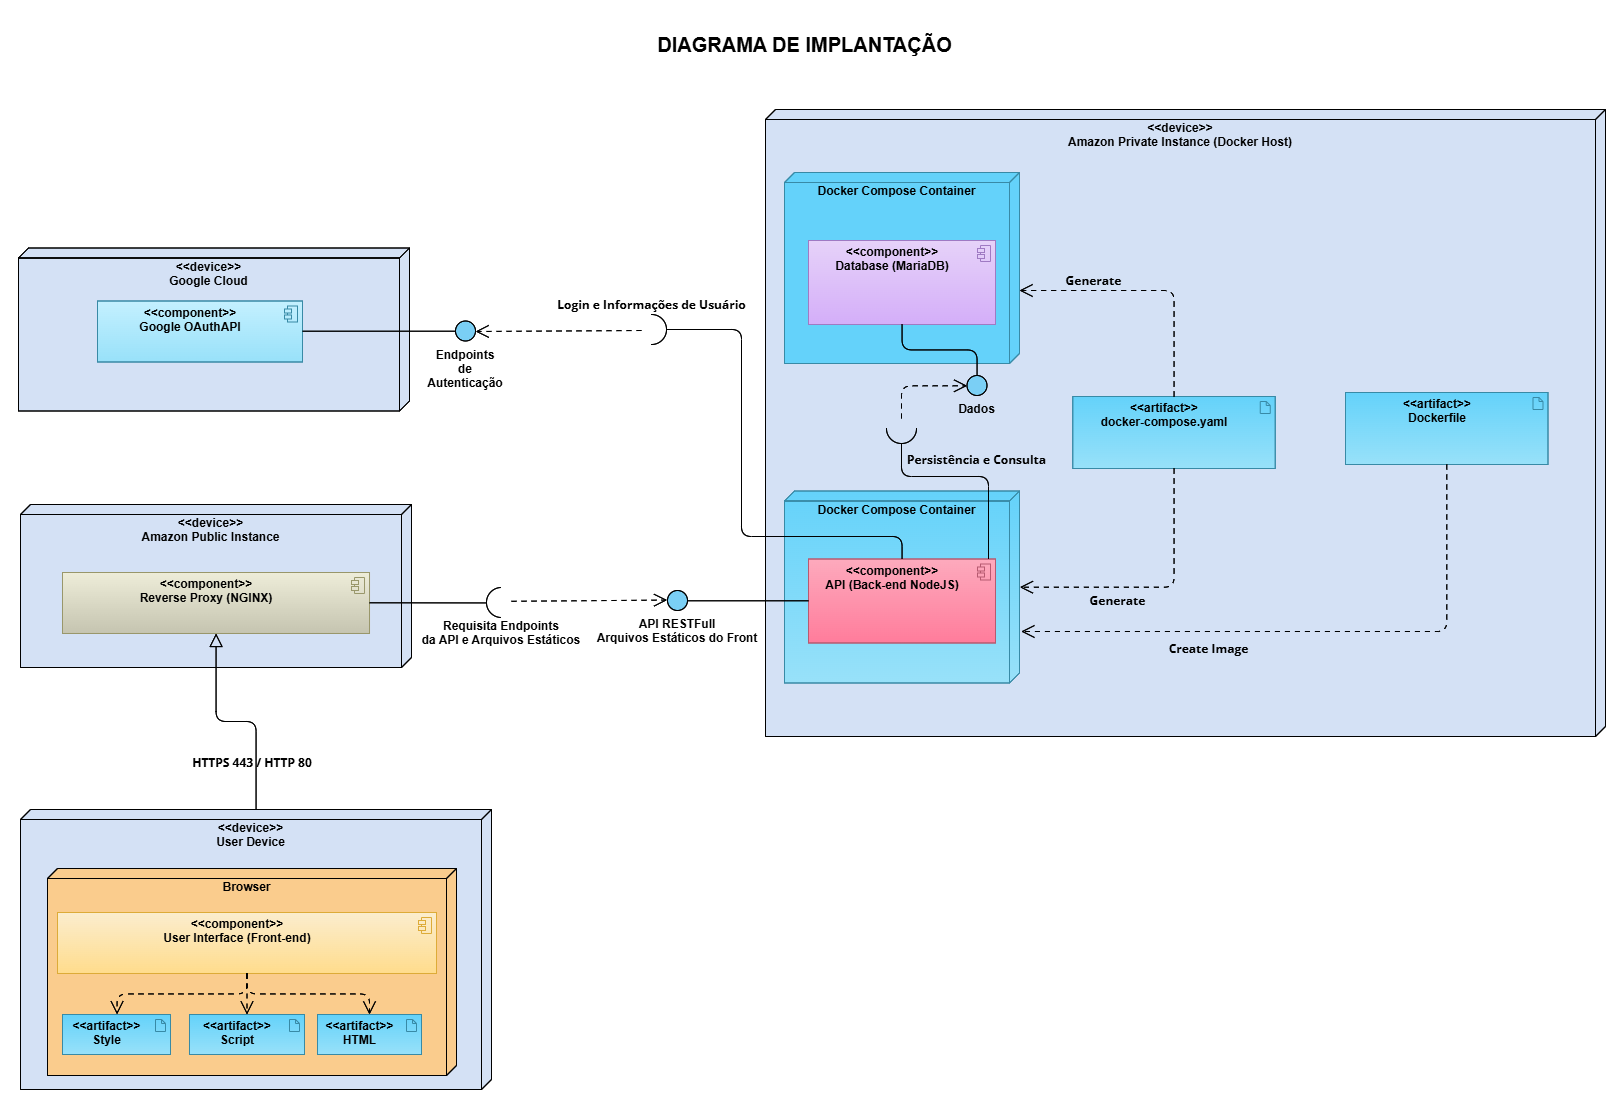
\includegraphics[width=\textwidth]{cap04-desenvolvimento/images/4-3-2-2-diagrama-implantacao}
  \caption{Diagrama de componente da aplicação}
  \label{fig:diagrama-implantacao}
\end{figure}

\subsubsection{Diagrama Geral}

Com o objetivo de fornecer uma visão mais aprofundada da infraestrutura da aplicação na nuvem, o Diagrama Geral apresenta a disposição dos principais componentes implantados na arquitetura da Amazon Web Services (AWS). 

Este diagrama ilustra elementos de infraestrutura fundamentais como sub-redes públicas e privadas, resolução de DNS, Virtual Private Cloud (VPC), Bastion Server, NAT Gateway, Internet Gateway, banco de dados, entre outros recursos. A representação facilita a compreensão técnica da topologia de rede e da distribuição dos serviços, evidenciando como a aplicação foi projetada para atender requisitos de segurança, escalabilidade e disponibilidade no ambiente da AWS.

\begin{figure}[htb]
  \centering
  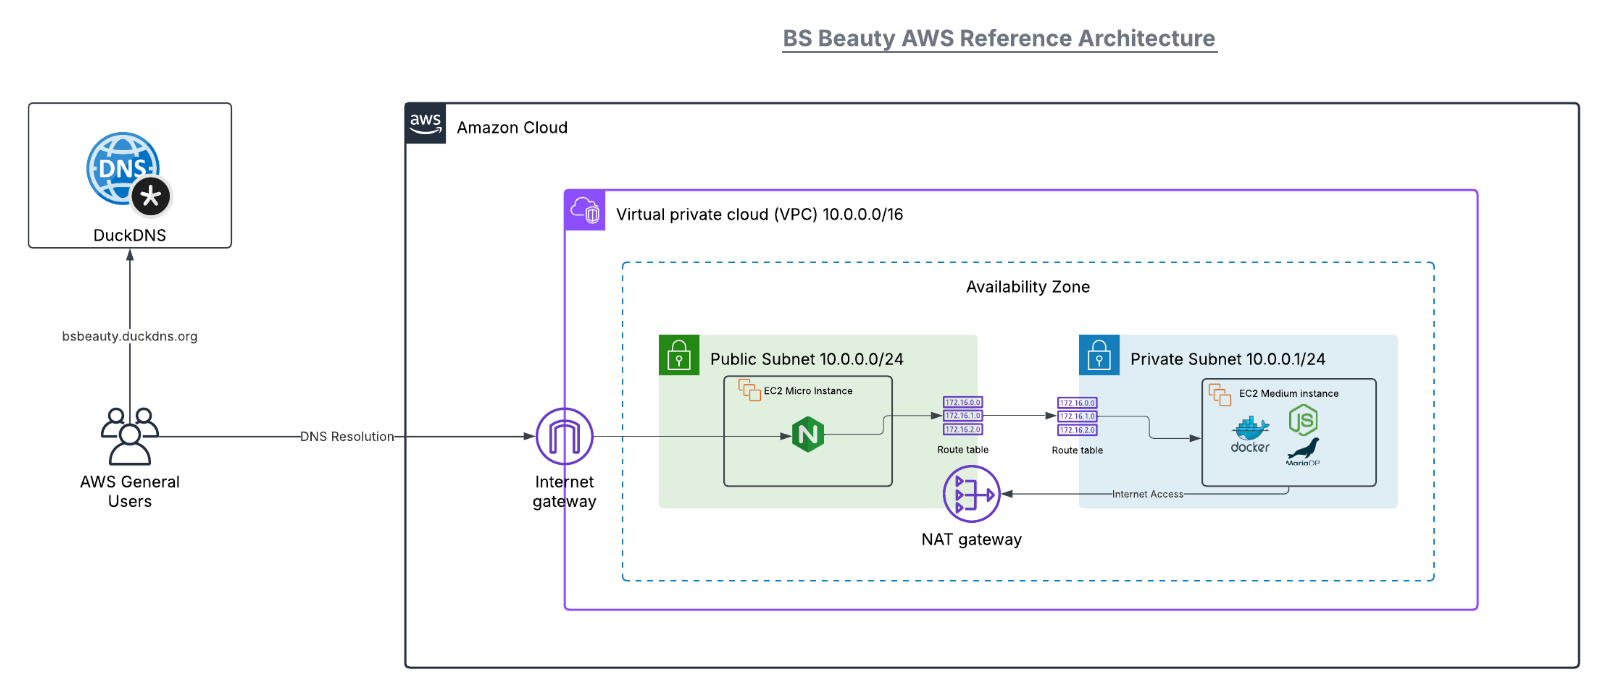
\includegraphics[width=\textwidth]{cap04-desenvolvimento/images/4-3-2-3-diagrama-geral}
  \caption{Diagrama Geral da Arquitetura}
  \label{fig:diagrama-geral}
\end{figure}
